%----------------------------------------------------------------------------------------
%	PACKAGES AND THEMES
%----------------------------------------------------------------------------------------

\documentclass{beamer}

\mode<presentation> {

\usetheme{Madrid}

}


\usepackage{graphicx} % Allows including images
\usepackage{booktabs} % Allows the use of \toprule, \midrule and \bottomrule in tables

\usepackage[normalem]{ulem} % strike text

%%% Вставка кода

\usepackage{listings}

%%% Работа с русским языком
\usepackage[T2A]{fontenc}			% кодировка
\usepackage[utf8]{inputenc}			% кодировка исходного текста
\usepackage[english]{babel}	% локализация и переносы




%%% Работа с картинками
\setlength\fboxsep{3pt} % Отступ рамки \fbox{} от рисунка
\setlength\fboxrule{1pt} % Толщина линий рамки \fbox{}
\usepackage{wrapfig} % Обтекание рисунков текстом

%%% Оформление стихов
\usepackage{verse}


\AtBeginSection[]
{
  \begin{frame}
    \frametitle{Содержание}
    \tableofcontents[currentsection]
  \end{frame}
}


%----------------------------------------------------------------------------------------
%	TITLE PAGE
%----------------------------------------------------------------------------------------

\title[Занятие 1]{Формальный анализ стиха. Занятие 1} % The short title appears at the bottom of every slide, the full title is only on the title page

\author{Борис Орехов} % Your name
\institute[НИУ ВШЭ] % Your institution as it will appear on the bottom of every slide, may be shorthand to save space
{
НИУ Высшая школа экономики \\ % Your institution for the title page
\medskip
\textit{nevmenandr@gmail.com} % Your email address
}
\date{8 сентября 2015} % Date, can be changed to a custom date

\begin{document}

\lstset{ %
language=Python,                 % выбор языка для подсветки (здесь это С)
basicstyle=\small\sffamily, % размер и начертание шрифта для подсветки кода
numbers=left,               % где поставить нумерацию строк (слева\справа)
numberstyle=\tiny,           % размер шрифта для номеров строк
stepnumber=1,                   % размер шага между двумя номерами строк
numbersep=1pt,                % как далеко отстоят номера строк от подсвечиваемого кода
backgroundcolor=\color{white}, % цвет фона подсветки - используем \usepackage{color}
showspaces=false,            % показывать или нет пробелы специальными отступами
showstringspaces=false,      % показывать или нет пробелы в строках
showtabs=false,             % показывать или нет табуляцию в строках
tabsize=2,                 % размер табуляции по умолчанию равен 2 пробелам
captionpos=t,              % позиция заголовка вверху [t] или внизу [b] 
breaklines=true,           % автоматически переносить строки (да\нет)
breakatwhitespace=false, % переносить строки только если есть пробел
escapeinside={\%*}{*)}   % если нужно добавить комментарии в коде
}

\begin{frame}
\titlepage % Print the title page as the first slide
\end{frame}



\begin{frame}
\frametitle{Содержание}  % Table of contents slide, comment this block out to remove it
\tableofcontents % Throughout your presentation, if you choose to use \section{} and \subsection{} commands, these will automatically be printed on this slide as an overview of your presentation
\end{frame}

%----------------------------------------------------------------------------------------
%	PRESENTATION SLIDES
%----------------------------------------------------------------------------------------



%------------------------------------------------
\section{Что такое стихи}\label{sec:intro} % Sections can be created in order to organize your presentation into discrete blocks, all sections and subsections are automatically printed in the table of contents as an overview of the talk
%------------------------------------------------

\subsection{Зачем пишут стихи}\label{sec:why} % A subsection can be created just before a set of slides with a common theme to further break down your presentation into chunks

%------------------------------------------------

\begin{frame}
\frametitle{Зачем пишут стихи}
По всей видимости, написание стихов — это социальная деятельность, отличная у профессиональных и наивных авторов.
Наивные авторы считают, что
\begin{itemize}
\item стихи — это престижный способ выражения их эмоций;
\item достаточно соблюсти минимум требований к поэтическому тексту, чтобы он стал литературным:
\begin{itemize}
\item ритм;
\item рифма;
\item тематический набор (про любовь);
\end{itemize}
\end{itemize}

\begin{verse}
Как он мог так со мной поступить –\\
Ведь любила его всей душою!\\
Так хотела я рядом с ним быть,\\
Только бросил меня и ушел он.\\
\end{verse}

\end{frame}

%------------------------------------------------

\begin{frame}
\frametitle{Являются ли стихи выразителями «души»}
«Анна Андреевна заговорила со мной о Б., нашей студентке, которая приходила к ней читать плохие стихи, ссылаясь, между прочим, на то, что она моя и Гуковского ученица.

Я: “Б. говорила мне, что пишет стихи. Но она предупредила меня, что это, собственно, не стихи, а откровения женской души, и я, убоявшись, не настаивала”.

А. А. (ледяным голосом): “Да, знаете, когда в стихах дело доходит до души, то хуже этого ничего не бывает”».

\textit{Лидия Гинзбург}

\begin{flushleft}
По всей видимости, образ вдохновенного поэта, ставящего целью описать свои чувства, довольно поздний и восходит к эпохе романтизма (рубеж XVIII—XIX веков).
\end{flushleft}


\end{frame}

%------------------------------------------------

\begin{frame}
\frametitle{А для профессиональных авторов?}
\begin{flushleft}
Прежде всего, стихи — это сложно организованные объекты, определённым образом взаимодействующие с традицией, с уже написанным раньше.
\end{flushleft}


М. Л. Гаспаров:

«Главная же диалектическая противоположность, делающая текст стихотворения живым, в том, что этот текст представляет собой поле напряжения между нормой и ее нарушениями. При чтении стихотворения (а тем более — многих стихотворений одной поэтической культуры) у читателя складывается система ожиданий: если стихотворение начато пушкинским ямбом, то ударения в нем будут ожидаться на каждом втором слоге, а лексика будет возвышенная и (для нас) слегка архаическая, а образы в основном из романтического набора и т. д.»
\end{frame}

%------------------------------------------------

\begin{frame}
\frametitle{Норма и её нарушения}
М. Л. Гаспаров:

«Эти ожидания на каждом шагу то подтверждаются, то не подтверждаются: в ямбе ударения то и дело пропускаются, про смерть Ленского после романтического “Потух огонь на алтаре!” вдруг говорится: “…как в доме опустелом… окна мелом забелены…” и т. п. Именно подтверждение или неподтверждение этих читательских ожиданий реальным текстом ощущается как эстетическое переживание. Если подтверждение стопроцентно, (“никакой новой информации”), то стихи ощущаются как плохая, скучная поэзия; если стопроцентно неподтверждение (“новая информация не опирается на имеющуюся”), то стихи ощущаются как вообще не поэзия”». 
\end{frame}

%------------------------------------------------

\begin{frame}
\frametitle{Текст и традиция}
\begin{itemize}
\item Таким образом, профессиональный автор будет заботиться не о том, чтобы точнее или полнее выразить свои эмоции в тексте, а о том, чтобы это выражение определённым образом соотносилось с традицией, уже написанным. 

\item «Красота» (эстетическая категория прекрасного), по всей видимости, вторична по отношению к прочитанному. В очень редких случаях эстетический объект может вызывать эффект вне связи с контекстом.

\item В одной современной антиутопии уничтожают картины, чтобы они не вызывали эмоции. Это неправдоподобно!

\end{itemize}

\end{frame}

%------------------------------------------------

\begin{frame}
\frametitle{Текст и традиция}

\begin{verse}
\color{red}{Я памятник себе воздвиг} \color{black}нерукотворный,\\
К нему не зарастет народная тропа,\\
Вознесся \color{green}{выше} \color{black}он главою непокорной\\
\color{green}{Александрийского столпа}.
\end{verse}

\begin{flushleft}
\color{black}{\large vs.}
\end{flushleft}

\begin{verse}
\color{red}{Я памятник себе воздвиг} \color{black}чудесный, вечный,\\
Металлов тверже он и \color{green}{выше пирамид};\\
\color{black}Ни вихрь его, ни гром не сломит быстротечный,\\
И времени полет его не сокрушит.
\end{verse}

\end{frame}

%------------------------------------------------

\subsection{Стихи и проза}\label{sec:diff}

%------------------------------------------------

\begin{frame}
\frametitle{Немного про термины}
\begin{itemize}
\item стих — ? 
\begin{itemize}
\item то, что не проза
\item одна строка стихотворного произведения
\end{itemize}
\item \sout{стих как «стихотворение»}
\end{itemize}
\end{frame}

%------------------------------------------------

\begin{frame}
\frametitle{Господин Журден}

\textbf{Г-н Журден}. А теперь я должен открыть вам секрет. Я влюблен в одну великосветскую даму, и мне бы хотелось, чтобы вы помогли мне написать ей записочку, которую я собираюсь уронить к ее ногам. <...>

\textbf{Учитель философии}.  Вы хотите написать ей стихи?

\textbf{Г-н Журден}. Нет, нет, только не стихи.

\textbf{Учитель философии}. Вы предпочитаете прозу?

\textbf{Г-н Журден}. Нет, я не хочу ни прозы, ни стихов.

\textbf{Учитель философии}. Так нельзя: или то, или другое.

\textbf{Г-н Журден}. Почему?

\textbf{Учитель философии}. По той причине, сударь, что мы можем излагать свои мысли не иначе, как прозой или стихами.

\textbf{Г-н Журден}. Не иначе, как прозой или стихами?

\textbf{Учитель философии}. Не иначе, сударь. Все, что не проза, то стихи, а что не стихи, то проза.
<...>

\textbf{Г-н Журден}. Честное слово, я и не подозревал, что вот уже более сорока лет говорю прозой. Большое вам спасибо, что сказали.

\end{frame}

%------------------------------------------------

\begin{frame}
\frametitle{Стих и проза}
Поэзия и проза отличаются друг от друга

\begin{itemize}
\item по статусу (или имиджу)
\item структурно
\end{itemize}

Расхожее представление состоит в том, что стихи труднее писать, следовательно, они являются более престижной формой речи (хотя хорошую прозу писать не легче).

Кроме того, стихотворная форма исторически связана с магическими практиками

\end{frame}

%------------------------------------------------

\begin{frame}
\frametitle{Структурные отличия стихов от прозы. Тупиковые варианты}

\begin{itemize}
\item ритм
\item рифма
\item цветы и птицы
\end{itemize}

\end{frame}

%------------------------------------------------

\begin{frame}
\frametitle{Ритм?}

А что такое ритм?
\begin{itemize}
\item ритм — последовательность повторяющихся или варьирующихся элементов
\end{itemize}

\begin{center}
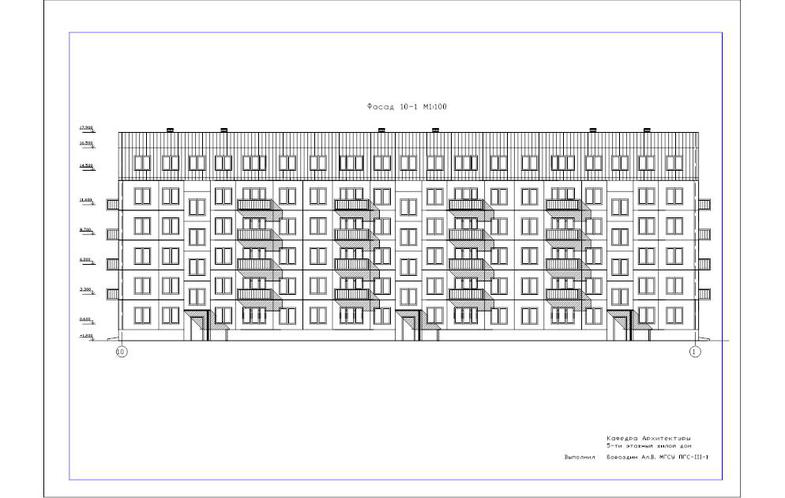
\includegraphics[width=0.7\textwidth]{building.png}
\end{center}

\end{frame}

%------------------------------------------------

\begin{frame}
\frametitle{Ритм?}

Ритм — универсальное понятие, он есть и в прозе

 Все \color{blue}счастливые семьи \color{black}похожи друг на друга, каждая \color{blue}несчастливая семья \color{black}несчастлива по-своему.
   \colorbox{gray}{Все смешалось} в доме Облонских. \colorbox{gray}{Жена узнала}, что \colorbox{gray}{муж был в связи} с бывшею в их доме француженкою-гувернанткой, и объявила мужу, что не может жить с ним в одном доме. \colorbox{gray}{Положение это продолжалось} уже третий день и мучительно чувствовалось и самими супругами, и всеми членами семьи, и домочадцами.

\end{frame}

%------------------------------------------------

\begin{frame}
\frametitle{Стихотворный ритм?}
\begin{flushleft}
Может быть, различению может служить «специальный» традиционно понимаемый стихотворный ритм?
\end{flushleft}

\begin{verse}
Она пришла с мороза,\\
Раскрасневшаяся,\\
Наполнила комнату\\
Ароматом воздуха и духов,\\
Звонким голосом\\
И совсем неуважительной к занятиям\\
Болтовней.\\
Она немедленно уронила на пол\\
Толстый том художественного журнала,\\
И сейчас же стало казаться,\\
Что в моей большой комнате\\
Очень мало места.\\
Все это было немножко досадно\\
И довольно нелепо.
\end{verse}

\end{frame}

%------------------------------------------------

\begin{frame}
\frametitle{Верлибр}

\begin{verse}
Впрочем, она захотела,\\
Чтобы я читал ей вслух «Макбета».\\
Едва дойдя до пузырей земли,\\
О которых я не могу говорить без волнения,\\
Я заметил, что она тоже волнуется\\
И внимательно смотрит в окно.\\
Оказалось, что большой пестрый кот\\
С трудом лепится по краю крыши,\\
Подстерегая целующихся голубей.\\
Я рассердился больше всего на то,\\
Что целовались не мы, а голуби,\\
И что прошли времена Паоло и Франчески.\\

1908
\end{verse}

\end{frame}

%------------------------------------------------

\begin{frame}
\frametitle{Рифма?}

\begin{verse}
In nova fert animus mutatas dicere formas\\
corpora; di, coeptis (nam vos mutastis et illas)\\
adspirate meis primaque ab origine mundi\\
ad mea perpetuum deducite tempora carmen.
\end{verse}

\begin{center}
Оно же:
\end{center}

\begin{verse}
Ныне хочу рассказать про тела, превращенные в формы\\
Новые. Боги, — ведь  вы превращения эти вершили, —\\
Дайте ж замыслу ход и мою от начала вселенной\\
До наступивших времен непрерывную песнь доведите
\end{verse}

\end{frame}

%------------------------------------------------

\begin{frame}
\frametitle{Тематика}

Р. О. Якобсон:

В эпоху классицизма или романтизма репертуар поэтических тем был весьма ограничен. Мы все хорошо помним традиционный реквизит: месяц, озеро, соловей, скалы, розы, замок и т.д. и т.п. Даже сны романтика не выходили за рамки этого круга. <...>  Особенно готические окна были в моде, и за ними обязательно светила луна. Сейчас для поэта одинаково поэтично любое окно, начиная с огромной зеркальной витрины универмага и кончая окошком деревенского трактира, густо засиженным мухами. 

\end{frame}

%------------------------------------------------

\begin{frame}
\frametitle{Тематика}

И через поэтические окна ныне можно увидеть всякое. Незвал писал об этом:

\begin{verse}
Посреди фразы меня вдруг ослепит сад\\
или нужник неважно что\\
я уже не различаю предметы по приписываемой им вами прелести или\\
безобразию.
\end{verse}


\end{frame}

%------------------------------------------------

\begin{frame}
\frametitle{Знаете ли вы венгерский?}

\begin{flushleft}
Hallgass, bújj el, s titkold, tagadd 

érzéseid, álmaidat! 

Mint fénylő csillagmiriád 

szállhatnak a lelkeden át, 

érkezve s tűnve, mint az éj: 

csodáld őket és - ne beszélj!

\end{flushleft}

\begin{flushleft}

Szív hol s kinek nyílhatna meg? 

Ki értheti az életed? 

Ki érthetné, ki vagy, mi vagy? 

Hazudik a kész gondolat! 

Merítve sár a tiszta mély: 

igyál belőle s - ne beszélj!

\end{flushleft}

Это стихи или проза?


\end{frame}

%------------------------------------------------

\begin{frame}
\frametitle{А это?}

A Goldberg-variációk Bach egyetlen variációformában komponált műve, amelyet Hermann Karl von Keyserlingk gróf és csembalistája, Johann Gottlieb Goldberg számára írt 1741–42-ben. A mű átfogó, akadémikus alkotás, a barokk variációművészet mintapéldája. Minden rész önálló karakterrel, egyedi hangulattal bír, amelyek összhangját a tudatosan építkező szerkezet és az erőteljes, kánon alakzatokban rendszeresen visszatérő egyetlen közös basszustéma biztosítja.

A szokatlanul hosszú – 32 ütemes – főtéma harmóniameghatározó vázhangjai mind a harminc variációban változatlanok maradnak, míg az ívmotívum variált formákban ismétlődik meg. A műben háromféle variációtípus váltakozik: a fokozódó virtuozitással komponált futamokból, arpeggiókból álló „figuratív variációkat”, a különböző formák és műfajok stílusában – triószonáta, tánc, siciliano, fúga, szólóconcerto, ária, francia nyitány, quodlibet – felhangzó „karaktervariációk” követik, majd az ária basszustémája fölött egyre nagyobb belépési távolságokkal (a prímtől egészen a nonáig) megalkotott „kánonok” zárják. 

\end{frame}

%------------------------------------------------

\begin{frame}
\frametitle{Проза как телетайпная лента}

\begin{center}
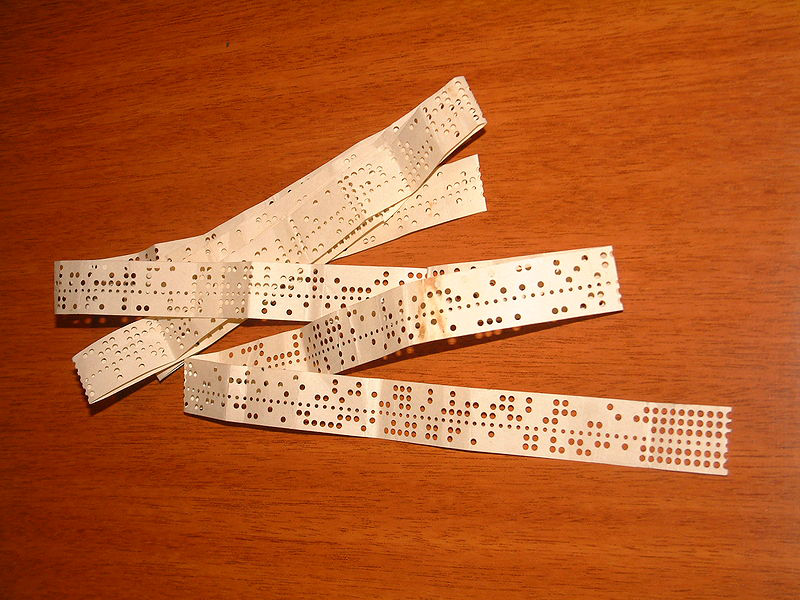
\includegraphics[width=0.8\textwidth]{lenta.png}
\end{center}

\end{frame}

%------------------------------------------------

\begin{frame}
\frametitle{Стихи как система парадигматических членений}

\begin{center}
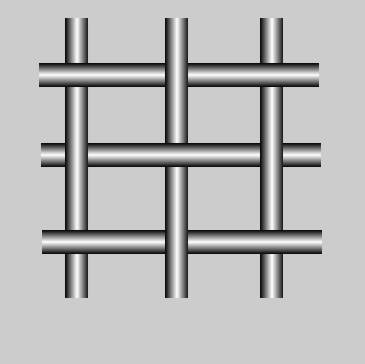
\includegraphics[width=0.3\textwidth]{reshetka.jpg}
\end{center}

\begin{verse}
Еще в полях белеет \color{red}снег, \\
\color{black}А воды уж весной \color{green}шумят – \\
\color{blue}Бегут \color{black}и будят сонный \color{red}брег, \\
\color{blue}Бегут \color{black}и блещут и \color{green}гласят\color{black}...
\end{verse}
\end{frame}

%------------------------------------------------

\begin{frame}
\frametitle{Определение}

{\Large Стих — это система сквозных принудительных парадигматических членений, структурирующих дополнительное измерение текста}

\begin{flushleft}
(М. И. Шапир)
\end{flushleft}

\end{frame}

%------------------------------------------------

\begin{frame}
\frametitle{Что не отменяет поэтических определений}

\poemtitle{Определение поэзии}
\begin{verse}
Это — круто налившийся свист,\\
Это — щелканье сдавленных льдинок.\\
Это — ночь, леденящая лист,\\
Это — двух соловьев поединок.

Это — сладкий заглохший горох,\\
Это — слезы вселенной в лопатках,\\
Это — с пультов и с флейт — Figaro\\
Низвергается градом на грядку.
\end{verse}

\end{frame}

%------------------------------------------------

\section{Зачем анализировать стихи}\label{sec:main}

%------------------------------------------------

%------------------------------------------------

\begin{frame}
\frametitle{Анализ стихов. Зачем?}

\begin{itemize}
\item Правда ли, что это не наука, если нет практической пользы?
\end{itemize}

\begin{itemize}
\item Познавание окружающего мира, видимо, базовое свойство человеческого сознания
\item Стихи существуют. И они довольно непонятная штука
\item От астрофизики тоже практической пользы немного
\end{itemize}

\end{frame}

%------------------------------------------------

\begin{frame}
\frametitle{Кто анализирует стихи?}

\begin{itemize}
\item Литературоведы
\item Лингвисты
\begin{itemize}
\item Стихи написаны на естественном языке
\item Лингвисты хорошо разбираются в том, как устроен язык
\end{itemize}
\end{itemize}

\end{frame}

%------------------------------------------------

\begin{frame}
\frametitle{«Что хотел сказать автор?»}

Правда ли, что этот вопрос интересует тех, кто анализирует стихи?

\begin{center}

{\Large Нет}

\end{center}

\begin{itemize}
\item Здесь не может быть применена модель «загадка—ответ»
\begin{itemize}
\item ответы принципиально множественны 
\item их правильность трудноверифицируема
\end{itemize} 
\item Непонятна цель такого подхода: почему мнение одного человека ценнее, чем другого
\item Тексты живут собственной жизнью, отдельно от автора
\end{itemize}

\end{frame}

%%------------------------------------------------

\section{Как анализируют стихи}\label{sec:main2}

%------------------------------------------------

\begin{frame}
\frametitle{Анализ стихов. Как?}


\begin{itemize}
\item Формально
\begin{itemize}
\item анализ языка
\item анализ метрики
\end{itemize} 
\item Неформально
\begin{itemize}
\item уровень смыслов
\item интертекстуальные связи
\end{itemize} 
\end{itemize}

\end{frame}

%------------------------------------------------

\begin{frame}[fragile]
\frametitle{Теснота стихового ряда}



Важная идея: каждый, даже самый минимальный, элемент художественного текста значим, оказывает влияние на всю структуру.

Сравним две программы

\begin{lstlisting}[label=example-code,caption=Первая программа]
line = raw_input()
new_line = line.split('.')
print new_line
\end{lstlisting}

\begin{lstlisting}[label=example-code2,caption=Вторая программа]
line = raw_input()
new_line = line.strip('.')
print new_line
\end{lstlisting}

Отличия в коде минимальны, но результат принципиально различен.

В стихах так же.

\end{frame}


%------------------------------------------------


\begin{frame}
\frametitle{Теснота стихового ряда}

\begin{itemize}
\item Это значит, что нельзя в других словах пересказать то же самое содержание.
\item В других словах это будет уже другое содержание (для художественного текста принципиально невозможно создать краткое содержание).
\item Лирический текст vs. нарратив. Иллюзия пересказа доступна только для нарратива. Попробуйте пересказать <<Шёпот. Робкое дыханье...>>
\end{itemize}



\end{frame}


%------------------------------------------------

\begin{frame}
\Huge{\centerline{продолжение следует}}
\end{frame}

%----------------------------------------------------------------------------------------

\end{document}